\documentclass{standalone}

\usepackage[OT1]{fontenc}
\renewcommand*\familydefault{\sfdefault}
\usepackage{helvet,sfmath}
\usepackage{siunitx}

\usepackage{tikz}
\usetikzlibrary{arrows,calc,patterns}
% \usetikzlibrary{intersections, calc, arrows.meta}
\usepackage{tikz,tkz-euclide}

\begin{document}
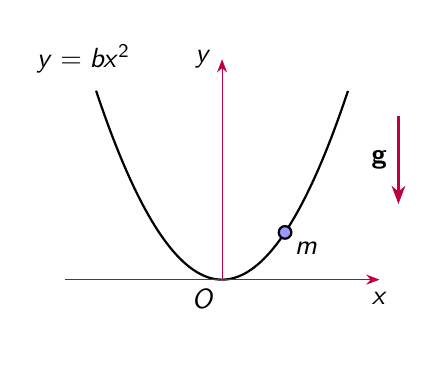
\begin{tikzpicture}[scale=0.8, >=Stealth]

    %% Background
    \draw[draw=none] (-3,-1) rectangle (3,4);

    % Parabol
    \draw[thick, domain=-2:2, samples = 100, smooth, variable=\t] 
    plot ({\t}, {0.75*\t*\t});
    \draw
    (-2.2,3.5) node{\(y = b x^2\)}
    ;

    % Particle
    \draw[thick, fill=blue!40] (1,0.75) circle (0.1);
    \draw
    (1,0.75) node[below right]{\(m\)}
    ;

    %Coordinate
    \draw[purple, -Stealth] (-2.5,0) to (2.5,0);
    \draw[purple, -Stealth] (0,0) to (0,3.5);

    \draw
    (-0.3,3.5) node{\(y\)}
    (2.5,-0.3) node{\(x\)}
    (-0.3,-0.3) node{\(O\)}
    ;

    %Gravity
    \draw[thick, purple, -Stealth] (2.8,2.6) to (2.8,1.2);
    \draw
    (2.5,1.9) node{\(\mathbf{g}\)}
    ;
    
\end{tikzpicture}
\end{document}